
\begin{enumerate}
\item 
\question{Take a look at the circuit in Figure~\ref{figSimple555Oscillator} (this will be used as the basis for the problems in this section).   Copy this circuit to a piece of paper.  Draw a line in one color showing how the current flows in the main circuit as it charges the capacitor.  With a different color, draw a line showing how current flows as the capacitor discharges.  Use arrows to indicate current direction.  You can ignore the ``Output'' and ``Control'' sections of the circuit for this problem.}
\solution{The lines should be drawn as follows:\newline
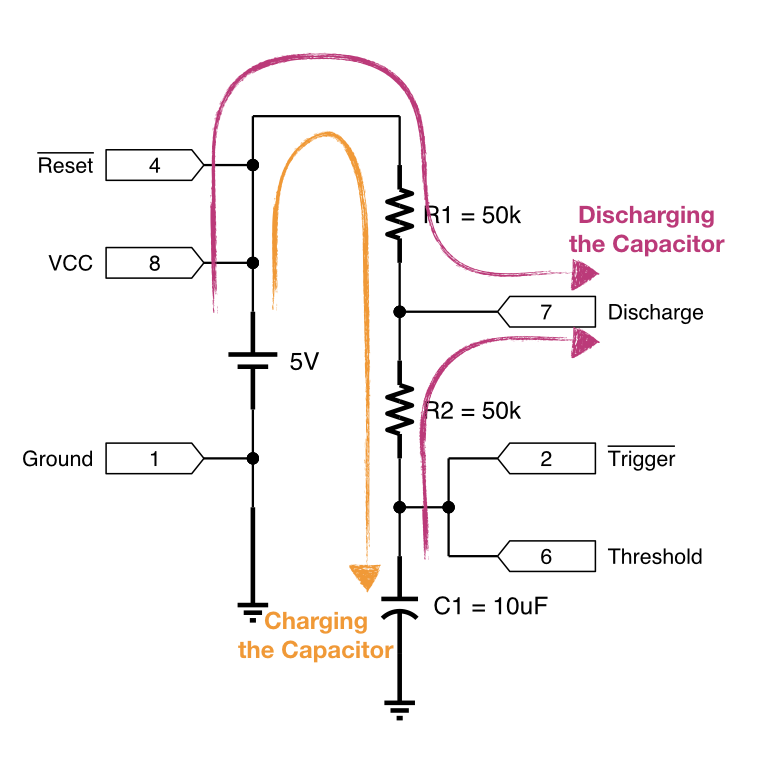
\includegraphics[width=0.8\columnwidth]{ExOscillatorChargeDischarge.png}
}
\explanation{
During the charging phase, current flows from the positive all the way into the capacitor.
This is shown with the line that is on the interior of the circuit.
During the discharge phase, Pin~7 goes low, and therefore current flows into Pin~7 from \emph{both}
the power supply \emph{and} from the capacitor.
}
\item 
\question{Why is R1 important?  What would happen if we just replaced it with a wire?}
\solution{During the discharge phase, R1 acts as a current-limiting resistor.  It would create a short-circuit from power to ground if it was just a wire.}
\explanation{Remember, there is no intelligence in a circuit.
The power supply only knows how to supply power.
Therefore, during the discharge phase, the power supply \emph{will continue to supply power just as before}.
When Pin~7 goes to zero volts, not only does the charge from the capacitor start to flow in that direction, but also the power from the supply.
If there is no resistor here, then it becomes a short-circuit from supply to ground.
Additionally, since this power is entirely wasted, R1 also limits the amount of waste that occurs during the discharge phase.
}
\item 
\question{Why are there two different pins on the NE555 connected to the capacitor?  What type of circuit (that we have discussed in this book) do you think they are connected to inside the chip?}
\solution{One compares for voltage \emph{above} a certain level, and the other compares for voltage \emph{below} a certain level.  Since they are checking for voltage, they are probably voltage comparator circuits.}
\explanation{The NE555, in its standard configuration, allows the capacitor to charge until it is two thirds full, and then discharges it until it is only one third full.
It has to detect for each of these conditions.
Therefore, it has two separate sensing inputs, one for each condition.  
$Threshold$ watches for the high voltage (and switches it from ``charge'' to ``discharge'' when it goes over), and $\overline{Trigger}$ watches for the low voltage (and switches it from ``discharge'' to ``charge'' when it goes under).
Since it is watching voltage levels, it is likely using a voltage comparator in the chip to measure these voltages.
}
\item 
\question{Why is the charging time of the NE555 always at least a little longer than the discharging time?}
\solution{The circuit uses both R1 and R2 to charge, but \emph{only} uses R2 to discharge.  Therefore, the resistance for discharging will always be less than the resistance for charging.}
\item 
\question{Why does the NE555 stay in the on state a little longer when the circuit is first turned on?}
\solution{Generally, the NE555 oscillates between filling and discharging the capacitor from one third to two-thirds full.  When first turned on, the capacitor will (presumably) be \emph{fully} discharged, so it will take some amount of time for that first charge cycle to occur, because it is charging from zero instead of from one third full.}
\item 
\question{Let's say that we wanted our circuit to be on for $2\mysec$ and off for $1\mysec$.  Keeping the same capacitor, what values should we use for R1 and R2 to accomplish that?}
\solution{R1 would be $144300.2\myohm$ and R2 would be $144300.1\myohm$.  In terms of standard components, using a $150\mykohm$ resistor for each one would be sufficient.}
\explanation{Since the discharge phase (when the output is off) only uses one resistor (R2) we will beging considering the discharge phase.
The total time is $1\mysec$.
Since we are using a NE555 timer, this time will cover $0.693$ time constants.
The time constant is given by the resistance multiplied by the capacitance.
Since the capacitor is a $10\myuf$ capacitor, the full equation is:
\begin{align*}
R \cdot 0.00001 \cdot 0.693 &= 1 \\
R &= \frac{1}{0.00001 \cdot 0.693} \\
R &\approx 144300.1
\end{align*}
Therefore, R2 will be approximately $144300.1\myohm$.
We now do a similar operation to find R1.  
However, the ``on'' phase of the oscillation will utilize both R1 and R2, and will take two seconds.
\begin{align*}
0.00001 \cdot (144300.1 + R) \cdot 0.693 &= 2 \\
144300.1 + R &= \frac{2}{0.00001 \cdot 0.693} \\
R &= \frac{2}{0.00001 \cdot 0.693} - 144300.1 \\
R &\approx 144300.2 
\end{align*}
Resistors are not actually available in these values.
Therefore, you would likely choose a $150\mykohm$ resistor for each of these.
}
\item 
\question{Let's say that we wanted our circuit to be on for $10\mysec$ and off for $3\mysec$.  Keeping the same capacitor, what values should we use for R1 and R2 to accomplish that?}
\item 
\question{The factory called and said that they were out of the capacitor we wanted for the circuit, and instead only had a $23\myuf$ capacitor that we could use.  Recalculate the previous problem using this new capacitor value.}
\item 
\question{How much current is our output sourcing from the chip?}
\item 
\question{When the chip first turns on (and thus the capacitor is empty and at $0\myvolt$) how much current is the RC circuit using?}
\end{enumerate}

% FIXME - might have a problem where people draw the pinout of the 555
% FIXME - might have a problem where they draw a circuit and then circle different part
